\section{Regularization}
    \subsection{The problem of overfitting}
    There are two types of errors in fitting functions to data, in which data shows the structure is not captured by the model. The terminology applies to both linear and logistic regression. Figure \ref{fig:fitting} shows an example of each fitting case. 

            \begin{enumerate}
                \item Underfitting (high bias): when the form of our hypothesis function ($h_\theta (x)$) maps poorly to the trend of data. It is usually caused by a function that is either too simple or uses too little features. 
                \item Overfitting (high variance): when hypothesis function learns the training set very well hence fits the available data but does not generalize well to predict new data, i.e fitting too many details. It is usually caused by a complicated function that creates a lot of unneccessary curves and angles unrelated to the data. 
            \end{enumerate}
        
            \begin{figure}[htbp]
                \centering
                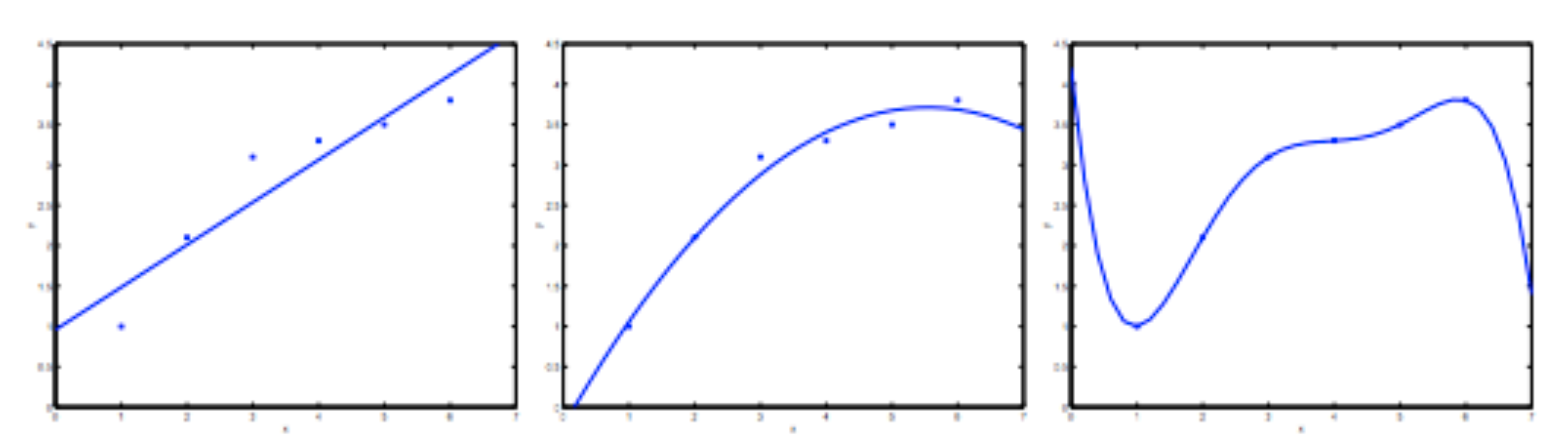
\includegraphics[width=\textwidth]{image/fitting.png}
                \caption{Three scenarios of fitting: underfit(left), good fit (middle), and overfit(right).}
                \label{fig:fitting}
            \end{figure}

        There are two main options to address the issue of overfitting:
            \begin{enumerate}
                \item Reduce the number of features
                    \begin{itemize}
                        \item manually select which features to keep.
                        \item Use a model selection algorithm (later in the course).
                    \end{itemize}
                \item \textbf{Regularization}
                    \begin{itemize}
                        \item Keep all the features, but reduce the magnitude of parameters $\theta_j$
                        \item Regularization worls well when we have a lot of slightly useful features. (Each contributes a bit to predict y)
                    \end{itemize}
            \end{enumerate}


    \subsection{Cost Function}
        \subsubsection{Intuition}
            Suppose we have overfitting, we can reduce the weight that some of the terms in our function carry by penalizing the feature parameter with increased cost. Consider the following hypothesis function : \[
            \theta_0 + \theta_1 x + \theta_2 x^2 + \theta x^3 + \theta x^4
        .\] We would want to make the function more quadratic, which means we would like to reduce the influence of $\theta_3$ and $\theta_4$. Since our goal was to minimize the cost function $J(\theta)$, we could modify the original cost function \[
            \min_\theta \frac{1}{2m} \sum_{i=1}^{m} ( h_\theta (x^{(i)}) - y^{(i)} )^2 + 1000\cdot \theta_3^2 + 1000\cdot \theta_4^2
        .\] This will force $\theta_3$ and $\theta_4$ to be close to zero, and make the original hypothesis function more quadratic.

        \subsubsection{Regularization}
            Now, we can take a step further and regularize all theta parameters: 

            \begin{equation}
                \min_\theta \:\:[ \frac{1}{2m} \sum_{i=1}^{m} ( h_\theta (x^{(i)}) - y^{(i)} )^2 ] + \lambda \sum_{j=1}^{n} \theta_j^2
                \label{eq:regularization-general-form}
            \end{equation}

            Here we are performing two separate operations which can be oberved as the two terms in Equation \ref{eq:regularization-general-form}. The first term corresponds to ``training the data'', and the second term relates to ``keeping the parameters small''. The coefficient $\lambda$ is the \textbf{regularization parameter} and determines the balance between the aforementioned two objectives. Note that if $\lambda$ is too big ($\approx$ 10\textsuperscript{10}), then all $\theta_j \approx 0$, except for $\theta_0$ (the constant term). This makes $h_\theta \approx 0$ and defies the purpose of training and leads to underfitting ( a flat horizontal line).




    \subsection{Regularized Linear Regression}
    \subsubsection{Gradient Descent} 
        We will modify the gradient descent function to separate out $\theta_0$ from the rest of the parameters because we do not want to penalize $\theta_0$.\\

        repeat until convergence\{  
            \[ \theta_0 := \theta_0 - \alpha \frac{1}{m} \sum_{i=1}^{m} ( h_\theta (x^{(i)}) - y^{(i)}) x_0^{(i)}\] 

            \[
                \theta_j := \theta_j - \alpha [ ( \frac{1}{m} \sum_{i=1}^{m} ( h_\theta (x^{(i)}) - y^{(i)}) x_j^{(i)} ) + \frac{\lambda}{m}\theta_j]
            \] 

        \} , where $j\in \{1, 2, \ldots, n\}$ \\

        The above equation can be re-arranged to get the final form:

        \begin{equation}
            \boxed{
            \theta_j := \theta_j (1-\alpha \frac{\lambda}{m}) - \frac{\alpha}{m} \sum_{i=1}^{m} ( h_\theta (x^{(i)}) - y^{(i)}) x_j^{(i)}
        }
            \label{eq:regularized-gradient-descent}
        \end{equation}

        The term $(1-\alpha \frac{\lambda}{m})$ will always be less than 1. Intuitively, this reduces the parameter, then the rest of equation \ref{eq:regularized-gradient-descent} carries the normal gradient descent.
        
        \subsubsection{Normal Equation}

        Recall from our previous normal equation (Equation \ref{eq:normal}), we have the design matrix \textbf{X} such that
            \[
            \mathbf{X} = \begin{bmatrix}
                \horzbar & (x^{(1)})^T & \horzbar \\
                \horzbar & (x^{(2)})^T & \horzbar \\
                \horzbar & (x^{(3)})^T & \horzbar \\
                         & \vdots      &          \\
                \horzbar & (x^{(m)})^T  & \horzbar \\
             \end{bmatrix}
            \]

            Now, to add in regularization to Equation \ref{eq:normal}, we get:

                 \begin{equation}
                     \boxed{
                     \mathbf{\theta} = (\mathbf{(X^TX)}+ \lambda\cdot\mathbf{L})^{-1} \mathbf{x}^Ty
                    }
                     \label{eq:regularized-normal}
                 \end{equation}

                 where $ L \in \mathbb{R}^{(n+1) \times (n+1)}$ 

                \begin{equation}
                    L = \begin{bmatrix}
                            0 & & & \\
                            & 1 & & \\
                            & &  \ddots & & \\
                            & &  & \ddots & \\
                            & & & & & 1 
                        \end{bmatrix}
                    \label{eq:regularized-L}
                \end{equation}
                
                Supopose non-invertibility arises: $m \leq n$, i.e \#examples is less than or equal to number of features, then using a $\lambda > 0$ in Equation \ref{eq:regularized-normal} will resolve the non-invertibility.



    \subsection{Regularized Logistic Regression}
            
        \subsubsection{Regularized Logistic Cost Function}
        We can modify our old logistic cost function (Equation \ref{eq:simplified-logistic-cost-function}) to apply regularization. 
                    \begin{equation}
                        \boxed{
                        J(\theta) = \frac{-1}{m} \, \sum_{i=1}^{m}\, [ y^{(i)}\, log\, h_\theta (x^{(i)})\; +\; (1-y^{(i)})\: log\:(\,1-h_\theta(x^{(i)})\,) ] + \frac{\lambda}{2m} \sum_{j=1}^{n} \theta_j^2
                    }
                        \label{eq:logistic-cost-function-regularized}
                    \end{equation}
                    Note that the second sum in Equation \ref{eq:logistic-cost-function-regularized} explicitly exludes the bias term $\theta_0$. 



        \subsubsection{Regularized Logistic Gradient Descent}
            The gradient descent is similar to that of linear regression; however note that the hypothesis function has been updated to Equation \ref{eq:log-reg-hypo}.\\

               repeat until convergence\{  
            \[ \theta_0 := \theta_0 - \alpha \frac{1}{m} \sum_{i=1}^{m} ( h_\theta (x^{(i)}) - y^{(i)}) x_0^{(i)}\] 

            \[
                \theta_j := \theta_j - \alpha [ ( \frac{1}{m} \sum_{i=1}^{m} ( h_\theta (x^{(i)}) - y^{(i)}) x_j^{(i)} ) + \frac{\lambda}{m}\theta_j]
            \] 

        \}




